\documentclass[11pt,letterpaper]{article}

\usepackage{../assets/scientific_report}
\usepackage{float}
\usepackage{listings}
\usepackage{xcolor}
\usepackage{graphicx}
\usepackage{geometry}
\usepackage{tikz}

\usetikzlibrary{shapes.geometric, arrows.meta, positioning}

\geometry{
    headheight=23pt,
    top=2cm,
    bottom=2cm,
    left=2.5cm,
    right=2.5cm
}

\setlength{\parskip}{0.5em}
\setlength{\parindent}{0pt}

\lstset{
    language=C,
    basicstyle=\ttfamily\small,
    keywordstyle=\color{blue}\bfseries,
    commentstyle=\color{green!60!black}\itshape,
    stringstyle=\color{red!80!black},
    numbers=left,
    numberstyle=\tiny\color{gray},
    numbersep=8pt,
    frame=single,
    breaklines=true,
    captionpos=b,
    tabsize=4,
    showstringspaces=false,
    inputencoding=utf8,
    extendedchars=true,
    literate={ã}{{\~a}}1 {õ}{{\~o}}1 {á}{{\'a}}1 {à}{{\`a}}1 {â}{{\^a}}1 {é}{{\'e}}1 {ê}{{\^e}}1 {í}{{\'i}}1 {ó}{{\'o}}1 {ô}{{\^o}}1 {ú}{{\'u}}1 {ç}{{\c{c}}}1 {Ã}{{\~A}}1 {Õ}{{\~O}}1 {Á}{{\'A}}1 {É}{{\'E}}1 {Í}{{\'I}}1 {Ó}{{\'O}}1 {Ô}{{\^O}}1 {Ú}{{\'U}}1 {Ç}{{\c{C}}}1
}

\begin{document}

\pagestyle{plain}

\begin{center}

{\LARGE\bfseries Mecanismos de Sincronização com OpenMP}\\[0.4em]

{\normalsize Eugenio Vitor Lopes dos Santos}\\[0.3em]

{\small DCA3703, Programação Paralela, Universidade Federal do Rio Grande do Norte}\\[0.3em]

\end{center}

\section{Enunciado}

Esta tarefa implementa o estimador de $\pi$ por Monte Carlo com
$N$ pontos uniformes em $[-1,1]^2$ e gerador \texttt{rand\_r} com
semente determinística por iteração. Cinco versões são comparadas:
(v1) contador compartilhado com \texttt{\#pragma omp critical} por hit,
(v2) contador compartilhado com \texttt{\#pragma omp atomic} por hit,
(v3) contador privado por thread com um único \texttt{critical} final,
(v4) vetor de parciais por thread com soma serial final e
(v5) cláusula \texttt{reduction}. Comparam-se desempenho e
produtividade de cada mecanismo e apresenta-se um roteiro direto
de quando utilizar cada um, incluindo \texttt{critical} nomeadas e
locks explícitos.

\section{Fundamentação teórica}

\subsection{Monte Carlo e semente por iteração}

O estimador utiliza

\[
\hat{\pi}=4\cdot\frac{n_{\mathrm{dentro}}}{N},
\]

com pontos uniformemente distribuídos em $[-1,1]^2$.

Para isolar o custo de sincronização, cada iteração $i$ gera uma semente
determinística própria:

\begin{center}
\texttt{seed = 12345u + i*2654435761u}
\end{center}

Esse procedimento, adotado nesta tarefa, emprega o hash
de Knuth e extrai $x$ e $y$ por meio de duas chamadas a
\texttt{rand\_r(\&seed)}.

Assim, o mesmo valor de $N$ produz os mesmos pontos e o mesmo valor de
\texttt{hits} com 1 ou 28 threads e em todas as versões (v1 a v5),
sem misturar o efeito do gerador de números aleatórios com o efeito da
sincronização.

\subsection{\texttt{critical}, \texttt{atomic} e \texttt{reduction}}

\texttt{critical} serializa um bloco estruturado qualquer utilizando
um mecanismo interno de exclusão mútua. O mecanismo pode proteger
qualquer conjunto de operações, mas cada entrada na região crítica
possui um custo de sincronização.

\texttt{atomic} cobre uma única operação escalar de
leitura-modificação-escrita, por exemplo, \texttt{hits++}, utilizando
uma operação atômica de hardware. Apresenta custo menor que
\texttt{critical} em operações simples, mas sua utilização é restrita
a um endereço e a uma operação compatível. O restante de uma expressão,
como \texttt{f()}, é executado fora da região atômica.

\texttt{reduction(+\:hits)} fornece a cada thread um acumulador privado
e realiza a combinação dos resultados ao final da região paralela.
O custo de combinação é da ordem de $O(p)$, em que $p$ representa o
número de threads, e o código necessário é mínimo.

O contador privado com \texttt{critical} final e o vetor por thread
com soma serial representam formas manuais do mesmo padrão, também
com custo de combinação da ordem de $O(p)$.

\subsection{Regiões críticas nomeadas e locks explícitos}

\texttt{critical(nome)} utiliza um nome literal que é resolvido pelo
compilador. Esse mecanismo é adequado para dois ou três recursos fixos,
como \texttt{lista0} e \texttt{lista1}.

Entretanto, essa abordagem não escala para $N$ recursos definidos em
tempo de execução, pois não é possível indexar diretamente uma região
crítica nomeada, como em:

\begin{lstlisting}[language=C,caption={Regiao critica nomeada nao indexavel}]
/* Invalido: o nome da regiao critica nao pode ser uma variavel. */
#pragma omp critical(locks[i])
    inserir(&heads[i], v);
\end{lstlisting}

Para $N$ dinâmico, utiliza-se um vetor de
\texttt{omp\_lock\_t locks[N]}, com as operações
\texttt{omp\_init\_lock}, \texttt{omp\_set\_lock},
\texttt{omp\_unset\_lock} e \texttt{omp\_destroy\_lock}.

Cada posição do vetor possui seu próprio lock, permitindo que recursos
distintos sejam acessados simultaneamente.

\section{Implementação}

Foram utilizadas cinco versões em C11, todas com cláusula
\texttt{default(none)} e medição de tempo com:

\begin{center}
\texttt{clock\_gettime(CLOCK\_MONOTONIC)}
\end{center}

\begin{itemize}

\item v1: contador compartilhado com \texttt{critical} por hit;

\item v2: contador compartilhado com \texttt{atomic} por hit;

\item v3: contador privado com \texttt{critical} uma única vez;

\item v4: vetor por thread com soma serial;

\item v5: \texttt{reduction(+\:hits)}.

\end{itemize}

A compilação foi realizada com as opções
\texttt{-std=c11 -O2 -Wall -fopenmp -lm}, utilizando
$N=2.000.000$.

\newpage
\begin{lstlisting}[language=bash,caption={Compilação e execução}]

gcc -std=c11 -O2 -Wall -fopenmp v1_shared_critical_randr.c -o pi_v1 -lm

gcc -std=c11 -O2 -Wall -fopenmp v2_shared_atomic_randr.c -o pi_v2 -lm

gcc -std=c11 -O2 -Wall -fopenmp v3_private_critical_randr.c -o pi_v3 -lm

gcc -std=c11 -O2 -Wall -fopenmp v4_vector_randr.c -o pi_v4 -lm

gcc -std=c11 -O2 -Wall -fopenmp v5_reduction_randr.c -o pi_v5 -lm

./execute.sh 2000000 3

\end{lstlisting}

\section{Resultados e discussão}

Foram avaliadas de 1 a 28 threads, com mediana de 3 repetições por
ponto, em um Intel i7-14700HX sob WSL2.

O valor de \texttt{hits} permaneceu idêntico em todas as versões e
para todas as quantidades de threads, demonstrando que a semente por
$i$ é reprodutível.

A versão v1 apresentou piora de desempenho com o aumento do número de
threads. Como a sincronização ocorre a cada hit, o tempo passou de
0,02~s com 1 thread para 0,48~s com 28 threads.

A versão v2 permaneceu relativamente estável, entre aproximadamente
0,03~s e 0,04~s. A operação atômica apresenta custo inferior ao de
\texttt{critical}, mas ainda ocorre sincronização a cada hit.

As versões v3, v4 e v5 apresentaram tempos entre 0,001~s e 0,002~s e
escalaram bem até 14 núcleos. Esse comportamento era esperado e
confirma que a privatização reduz significativamente o custo de
sincronização.

A Figura~\ref{fig:templog} resume o comportamento em escala
logarítmica, necessária porque v1 e v2 são ordens de grandeza mais
lentos que v3--v5. A tabela numérica e o gráfico em escala linear
foram suprimidos por redundância: repetiam os mesmos dados do gráfico
log sem permitir distinguir v3, v4 e v5. Os valores completos
permanecem disponíveis em \texttt{results.csv}.

\begin{figure}[H]

\centering


\includegraphics[width=0.95\textwidth]{tempo_execucao_log_plot.png}

\caption{Tempo de execução em função do número de threads, em escala
logarítmica, com $N=2.000.000$ e mediana de 3 repetições.}

\label{fig:templog}

\end{figure}

\section{Roteiro de uso}

A escolha do mecanismo de sincronização depende principalmente do tipo
de operação, da frequência de atualização e da quantidade de recursos
compartilhados.

O roteiro de decisão apresentado na Figura~\ref{fig:decisao} resume a
escolha do mecanismo mais adequado.

\begin{figure}[H]

\centering

\resizebox{0.92\textwidth}{!}{%
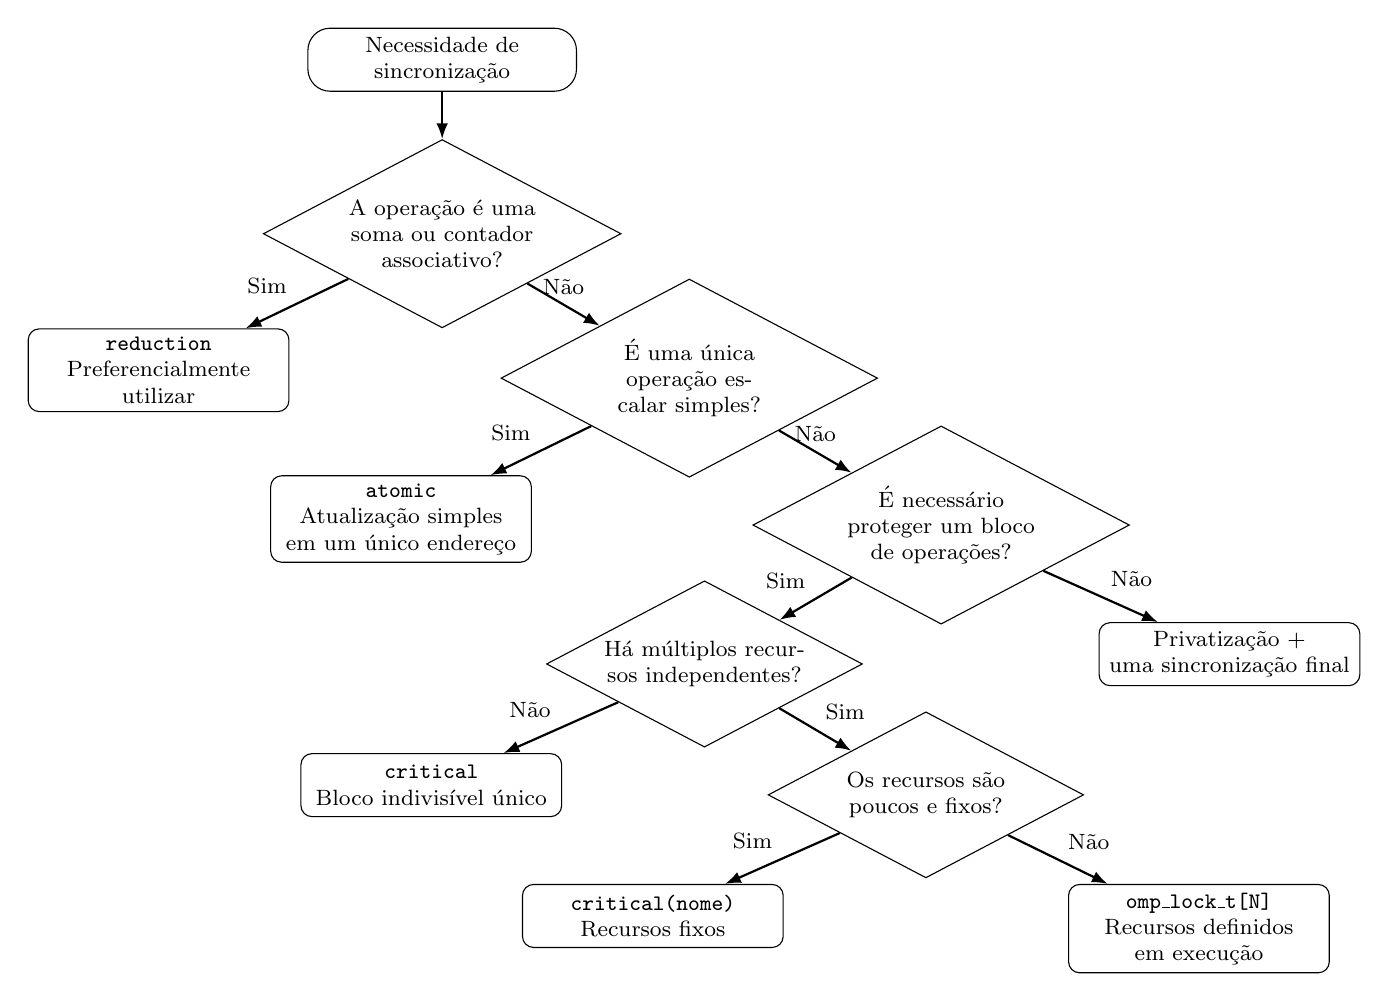
\begin{tikzpicture}[
    node distance=6mm and 8mm,
    every node/.style={
        font=\footnotesize,
        align=center
    },
    decision/.style={
        diamond,
        draw,
        aspect=1.9,
        text width=2.7cm,
        inner sep=1pt
    },
    process/.style={
        rectangle,
        draw,
        rounded corners,
        text width=3.1cm,
        minimum height=8mm,
        inner sep=3pt
    },
    startstop/.style={
        rectangle,
        draw,
        rounded corners=8pt,
        text width=3.2cm,
        minimum height=8mm,
        inner sep=3pt
    },
    line/.style={
        -{Latex[length=2mm]},
        thick
    },
    every edge quotes/.style={
        font=\scriptsize,
        inner sep=1pt
    }
]

\node[startstop] (inicio) {Necessidade de sincronização};

\node[decision, below=of inicio] (reducao)
    {A operação é uma soma ou contador associativo?};

\node[process, below left=of reducao] (reduction)
    {\texttt{reduction}\\
    Preferencialmente utilizar};

\node[decision, below right=of reducao] (simples)
    {É uma única operação escalar simples?};

\node[process, below left=of simples] (atomic)
    {\texttt{atomic}\\
    Atualização simples em um único endereço};

\node[decision, below right=of simples] (bloco)
    {É necessário proteger um bloco de operações?};

\node[decision, below left=of bloco] (multi)
    {Há múltiplos recursos independentes?};

\node[process, below left=of multi] (critical)
    {\texttt{critical}\\
    Bloco indivisível único};

\node[decision, below right=of multi] (fixo)
    {Os recursos são poucos e fixos?};

\node[process, below left=of fixo] (criticalnome)
    {\texttt{critical(nome)}\\
    Recursos fixos};

\node[process, below right=of fixo] (locks)
    {\texttt{omp\_lock\_t[N]}\\
    Recursos definidos em execução};

\node[process, below right=of bloco] (privado)
    {Privatização +\\
    uma sincronização final};

\draw[line] (inicio) -- (reducao);

\draw[line] (reducao) -- node[above left]{Sim} (reduction);
\draw[line] (reducao) -- node[above]{Não} (simples);

\draw[line] (simples) -- node[above left]{Sim} (atomic);
\draw[line] (simples) -- node[above]{Não} (bloco);

\draw[line] (bloco) -- node[above left]{Sim} (multi);
\draw[line] (bloco) -- node[above right]{Não} (privado);

\draw[line] (multi) -- node[above left]{Não} (critical);
\draw[line] (multi) -- node[above right]{Sim} (fixo);

\draw[line] (fixo) -- node[above left]{Sim} (criticalnome);
\draw[line] (fixo) -- node[above right]{Não} (locks);

\end{tikzpicture}% 
}

\caption{Diagrama de decisão para escolha do mecanismo de sincronização.}

\label{fig:decisao}

\end{figure}

De forma resumida, os mecanismos podem ser utilizados conforme os
seguintes critérios:

\begin{enumerate}

\item \texttt{reduction}: indicado para somas ou contadores associativos.
É o caminho mais curto e, neste caso, apresenta o melhor desempenho.

\item Privado + 1 sincronização final: redução manual quando o valor
combinado não é diretamente redutível, como no caso de múltiplas
variáveis ou inserção em uma estrutura compartilhada.

\item \texttt{atomic} por update: indicado para atualizações frequentes
em um único endereço e que possam ser expressas por uma operação
atômica simples.

\item \texttt{critical} por update: indicado quando é necessário proteger
um bloco contendo mais de uma operação que deve ser executada de forma
indivisível.

\item \texttt{critical(nome)}: indicado quando existem dois ou três
recursos fixos que precisam de mecanismos de exclusão mútua
independentes.

\item \texttt{omp\_lock\_t[N]}: indicado quando existem $N$ recursos e
essa quantidade é definida em tempo de execução.

\end{enumerate}

Como regra geral, recomenda-se realizar a sincronização por thread,
com custo da ordem de $O(p)$, em vez de realizar a sincronização por
hit, com custo da ordem de $O(N)$, salvo quando houver necessidade de
visibilidade imediata.

\section{Conclusão}

Para o método de Monte Carlo utilizado, \texttt{reduction} apresentou
o melhor equilíbrio entre desempenho e simplicidade. O mecanismo obtém
tempo semelhante ao das versões v3 e v4 com uma implementação mais
compacta, além de facilitar a leitura do código.

\texttt{atomic} apresentou desempenho superior ao de \texttt{critical}
quando utilizado por hit, aproximadamente 10 vezes melhor com
28 threads no cenário avaliado, mas ainda apresentou desempenho
inferior ao das abordagens baseadas em privatização.

A utilização de uma semente determinada pela iteração
permitiu realizar a comparação mantendo os mesmos pontos gerados em
todas as versões e quantidades de threads. Dessa forma, o efeito
observado nos tempos está relacionado principalmente ao mecanismo de
sincronização empregado.

Os valores numéricos completos encontram-se disponíveis em
\texttt{results.csv}.

\appendix
\section{Códigos-fonte das cinco versões}

Os listados abaixo correspondem aos arquivos compilados com
\texttt{-std=c11 -O2 -Wall -fopenmp -lm} e $N=2.000.000$.

\lstinputlisting[language=C,caption={v1: contador compartilhado com critical por hit. Versão base correta, porém lenta: cada hit serializa (O(N) entradas).},label={lst:v1}]{v1_shared_critical_randr.c}

\lstinputlisting[language=C,caption={v2: contador compartilhado com atomic por hit. Mesma corretude de v1, menor sobrecarga com instrução atômica.},label={lst:v2}]{v2_shared_atomic_randr.c}

\lstinputlisting[language=C,caption={v3: contador privado com critical final. Custo O(p): acumula sem lock, combina 1x por thread.},label={lst:v3}]{v3_private_critical_randr.c}

\lstinputlisting[language=C,caption={v4: vetor por thread com soma serial. Sem sincronização no laço; sem padding pode sofrer falso compartilhamento.},label={lst:v4}]{v4_vector_randr.c}

\lstinputlisting[language=C,caption={v5: reduction. Versão idiomática: o runtime cria cópias privadas e combina no fim.},label={lst:v5}]{v5_reduction_randr.c}

\end{document}